\documentclass{article}
\usepackage{amsmath, amssymb, tikz, geometry, graphicx, natbib, mwe, xcolor,
 listings, tabularx, pdfpages, blindtext, mathtools, stackengine, amsthm, pgfplots,bigints, relsize, upgreek, esint, array}
\usepackage{hyperref}
\usepackage{slashed, enumitem}

\pgfplotsset{width=10cm,compat=1.9}

\colorlet{myWhite}{white!35!gray}
\definecolor{shadeofgray}{HTML}{181818}
\definecolor{shadeofviolet}{HTML}{0f022c}

\hypersetup{
    colorlinks=true,
    linkcolor=violet,
    filecolor=magenta,      
    urlcolor=cyan,
    pdftitle={Overleaf Example},
    pdfpagemode=FullScreen,
}

\geometry{ 
 a4paper,
 total={170mm,257mm},
 left=20mm,
 top=10mm,
 }
 
\lstdefinestyle{mystyle}{ 
bracketsstyle=\color{red}
}

\title{Economia e Organizzazione Aziendale}
\author{Giuseppe Bumma}


%----------------------------------------------------------------------
%use this for a total black background
%\pagecolor{black}
%\color{myWhite}
%----------------------------------------------------------------------


\pagecolor{shadeofgray}
\color{myWhite}



\begin{document}

%Commands
\newcommand{\R}{\mathbb{R}}
\newcommand{\bb}[1]{\mathbb{#1}}
\newcommand{\cc}[1]{\mathcal{#1}}
\newcommand{ \lognormal }{\text{Lognormal} }
\newcommand{\tb}[1]{\textbf{#1}}
\newcommand*\circled[1]{\tikz[baseline=(char.base)]{%
            \node[shape=circle,draw,inner sep=2pt] (char) {#1};}}
%for using circled number in enumerate use:
%\begin{enumerate}[label=\protect\circled{\arabic*}]


\tableofcontents

\maketitle

\section{Introduzione alla contabilità}
\subsection{Cos'è un'azienda}
L'azienda è una organizzazione costituita da persone e da beni che, attraverso
una serie coordinata di operazioni, mira alla produzione e allo scambio di beni o
di servizi per soddisfare un bisogno.
\begin{itemize}
    \item \textbf{Definizione giuridica:} il codice civile (art. 2555) definisce azienda il complesso di beni
    organizzati da un soggetto (l'imprenditore), strutturato funzionalmente per
    l'esercizio dell'impresa (produzione di beni e servizi);
    \item \textbf{Definizione "economica":} istituto economico duraturo volto alla produzione di
    beni/servizi, per il soddisfacimento (diretto o indiretto) dei bisogni umani.
\end{itemize}


\subsubsection{Economia aziendale}
L'economia aziendale studia il ciclo
di vita e le condizioni di equilibrio
dell'azienda attraverso l'osservazione
dei fenomeni economici delle
aziende singole e dei loro aggregati; il \textit{sistema azienda} produce beni
per soddisfare i bisogni umani ed è
volto alla realizzazione degli obiettivi
del soggetto economico.
\vspace*{0.2cm}\\
Aspetti fondanti della gestione aziendale sono:
\begin{itemize}
    \item l'organizzazione aziendale;
    \item la gestione;
    \item la rilevazione e il controllo, attraverso l'analisi di \textbf{contabilità} e il controllo di gestione.
\end{itemize}



\subsection{La contabilità}
La Contabilità ha il fine di supportare
l'attività decisionale di chi governa
l'impresa e di tutti coloro che sono
interessati a conoscere le sue condizioni
economiche, finanziarie, patrimoniali. Sostanzialmente è il
processo di raccolta, misurazione, analisi,
interpretazione e comunicazione di
informazioni economiche e finanziarie che
consentano ai decisori di esprimere giudizi
e valutazioni sull'impresa.\\
Le informazioni sono necessarie agli \textit{shareholders}(azionisti, che sono effettivamente soci) e agli \textit{stakeholders} (coloro che hanno contatti con l'azienda, come clienti o fornitori)
\vspace*{0.1cm}\\
La contabilità ha le
seguenti caratteristiche: 
\begin{itemize}
    \item ha natura \textbf{tecnica}
    \item è guidata da regole;
    \item evolve in risposta ai cambiamenti
    economici e sociali.
\end{itemize}


\subsubsection{I concetti alla base
della contabilità}
I concetti o principi sono regole generali
che guidano l'azione, ma non prescrivono
esattamente come si debba registrare un
evento.
\vspace*{0.1cm}\\
I criteri alla base della formulazione dei
principi sono:
\begin{itemize}
	\item Rilevanza (di solito i costi di produzione)
    \item Oggettività
    \item Fattibilità
\end{itemize}
\noindent\fbox{%
\parbox{\linewidth}{%
\centering Il fine ultimo del processo contabile è la
produzione di \textbf{rendiconti economico-finanziari} \newline che sintetizzano il risulto della
gestione.
}%
}
\begin{center}
    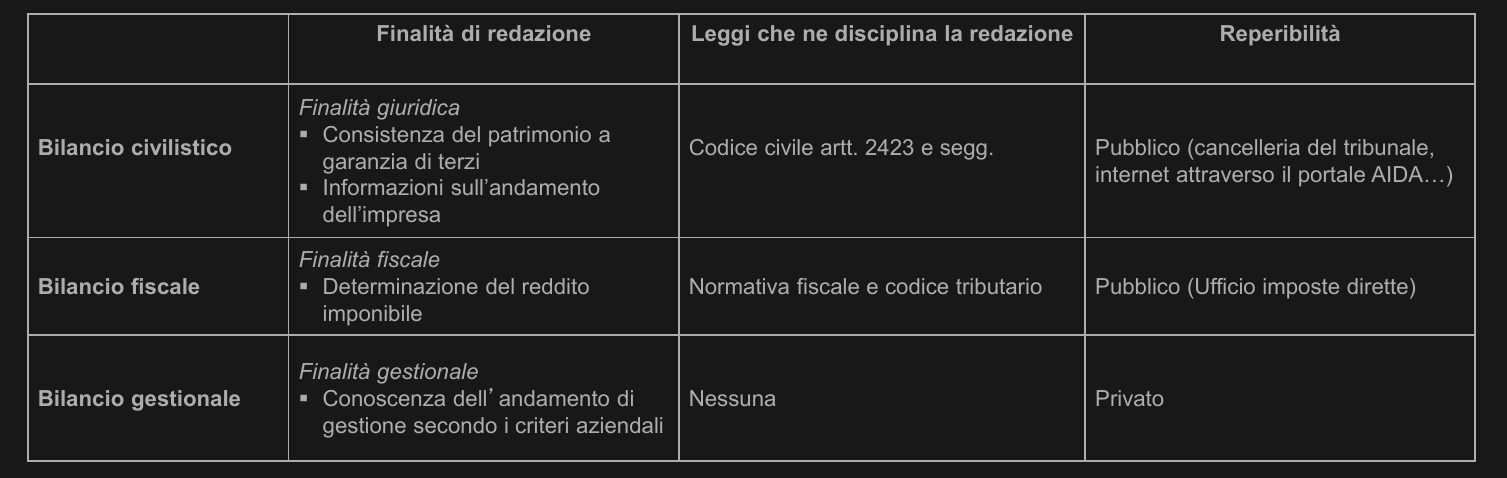
\includegraphics[scale=0.4]{Tabella bilancio.png}
\end{center}
\textbf{N.B.} Il bilancio fiscale si chiude sempre a dicembre, ma un'azienda può compilare un bilancio gestionale (con cadenza arbitraria, as es. mensile o bimestrale) per avere un'idea sui futuri investimenti.































\end{document}